\documentclass[12pt]{article}

\usepackage{amsmath, amssymb}
\usepackage[margin=1in]{geometry}
\usepackage{helvet}
\usepackage{tikz}
% \usepackage{figure}
\renewcommand{\familydefault}{\sfdefault}

\begin{document}
\def\assignment{Assignnment 3}

\pagenumbering{gobble}
\noindent{\large COSC 3020 \hfill Name: \underline{Jacob Tuttle} \\ Algorithms}
\begin{center}
    {\Large \assignment} \\ \textbf{\today}
\end{center}
\vspace{5pt}

\textbf{1. Dynamic Programming:} \texttt{held-karp.js} includes a memoized implementation of the Held-Karp algorithm for solving the traveling salesman problem. It can be accessed by including \texttt{const heldkarp = require('./held-karp.js');} in the beginning of another node.js file and then calling the function \texttt{heldkarp.tsp\_hk} and passing it a valid adjacency matrix. \\

The code was run on an Amazon Web Services t2.2xlarge linux instance using a set of randomized adjacency matrices. All times were rounded to the nearest whole second. Below, a figure plots the data points from graph sizes of 3 to 14. A graph of size 15 was left running for two hours without finishing, and so was stopped, putting the upper limit on this implementation of the Held-Karp algorithm running in under an hour at graphs of size 14. Extrapolating the data from the graph, we can estimate that a 15 node graph would take approximately 3.09 hours to complete; this represents a substantial jump in time from the 0.23 hours that were required to completely calculate the 14 node graph.
\begin{figure}[h]
    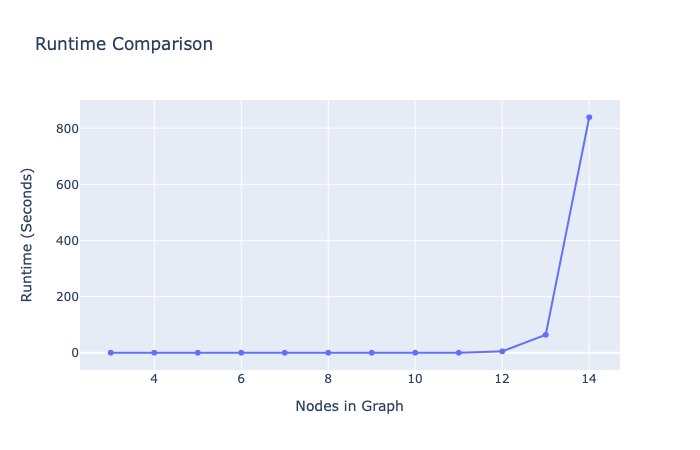
\includegraphics[width=\textwidth]{hk-comp.png}
\end{figure}

The worst case time complexity for this algorithm is the same as the best case since it will always calculate every possible path in order to determine which of them is the shortest. Therefore it has a time complexity of $O(2^n\cdot n^2)$. In order to store the sets of costs, we store all of these possible permutations of paths with a memory complexity of $O(2^n\cdot n)$.

\noindent\textbf{2. Stochastic Local Search:} 

\noindent\textbf{3. Comparison} and even more text. god damn.

\end{document}
